\documentclass[tikz,border=5pt]{standalone}
\usepackage[T1]{fontenc}
\usepackage{lmodern,amsmath,amssymb}
\usetikzlibrary{arrows.meta,calc,positioning,fit,backgrounds,shapes.geometric,matrix,decorations.pathreplacing,patterns}
\definecolor{ink}{gray}{0.08}
\definecolor{wash}{gray}{0.965}
\definecolor{soft}{gray}{0.45}
\tikzset{box/.style={draw=ink,line width=.65pt,fill=white,align=center,inner sep=4pt,outer sep=0pt,font=\small},flow/.style={draw=ink,line width=.65pt,-{Latex[length=1.8mm,width=1.3mm]},rounded corners=2pt},annotation/.style={font=\scriptsize,text=soft,align=center},groupbox/.style={draw=soft,dashed,line width=.45pt,fill=wash}}
\begin{document}
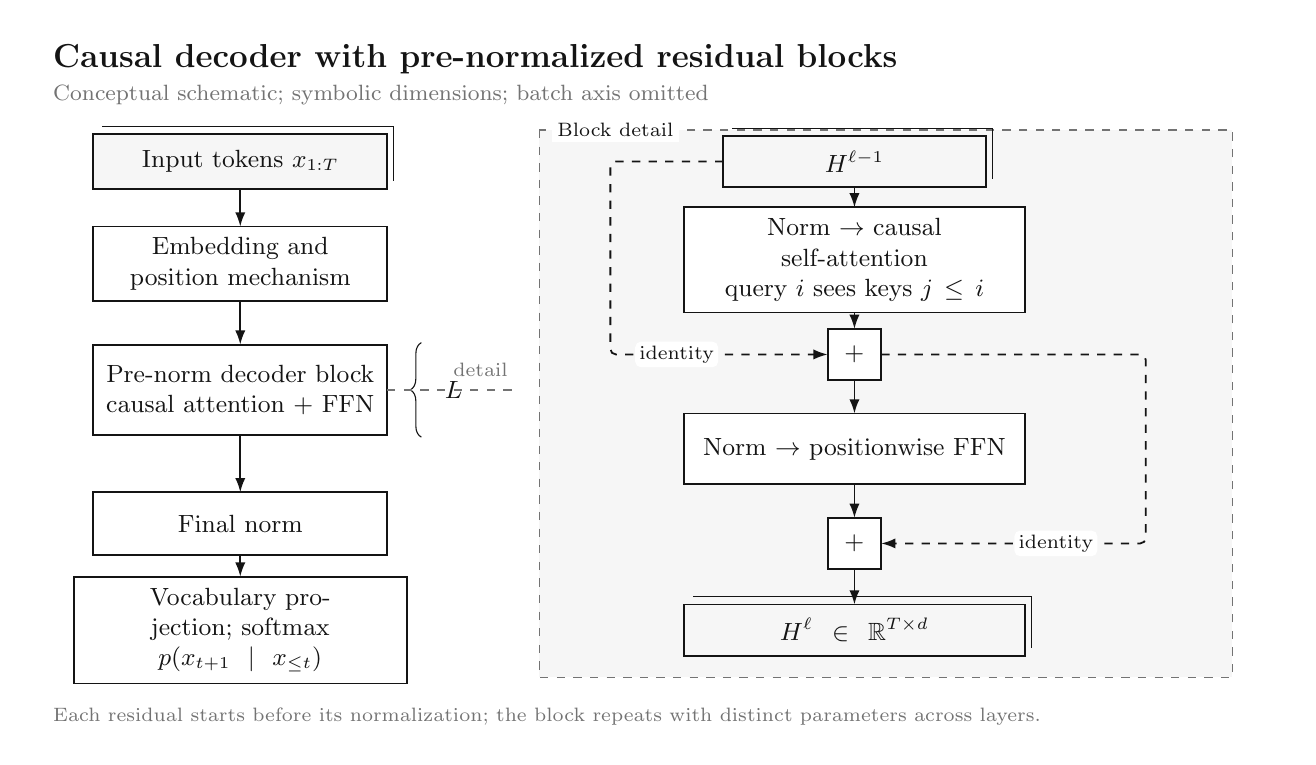
\begin{tikzpicture}[x=1cm,y=-1cm,font=\rmfamily,text=ink]

\path[use as bounding box] (0,0) rectangle (16,9);
\node[anchor=west,font=\large\bfseries] at (.2,.4) {Causal decoder with pre-normalized residual blocks};
\node[anchor=west,font=\footnotesize,text=soft] at (.2,.85) {Conceptual schematic; symbolic dimensions; batch axis omitted};
\begin{pgfonlayer}{background}
\draw[groupbox] (6.5,1.3) rectangle (15.3,8.25);
\node[anchor=west,font=\scriptsize,fill=white,inner sep=2pt] at (6.65,1.3) {Block detail};
\end{pgfonlayer}
\node[box,fill=wash,minimum width=3.7cm,minimum height=0.7cm,text width=3.45cm] (tokens) at (2.7,1.7) {Input tokens $x_{1:T}$};
\draw[ink,line width=.4pt] (0.9500000000000001,1.25) -- (4.65,1.25) -- (4.65,1.9499999999999997);
\node[box,minimum width=3.7cm,minimum height=0.9cm,text width=3.45cm] (embed) at (2.7,3.0) {Embedding and\\position mechanism};
\node[box,minimum width=3.7cm,minimum height=1.15cm,text width=3.45cm] (block) at (2.7,4.6) {Pre-norm decoder block\\causal attention $+$ FFN};
\node[box,minimum width=3.7cm,minimum height=0.8cm,text width=3.45cm] (norm) at (2.7,6.3) {Final norm};
\node[box,minimum width=4.2cm,minimum height=0.95cm,text width=3.95cm] (head) at (2.7,7.65) {Vocabulary projection; softmax\\$p(x_{t+1}\mid x_{\leq t})$};
\node[box,fill=wash,minimum width=3.3cm,minimum height=0.65cm,text width=3.05cm] (x) at (10.5,1.7) {$H^{\ell-1}$};
\draw[ink,line width=.4pt] (8.95,1.275) -- (12.25,1.275) -- (12.25,1.9249999999999998);
\node[box,minimum width=4.3cm,minimum height=1.0cm,text width=4.05cm] (attn) at (10.5,2.95) {Norm $\rightarrow$ causal self-attention\\query $i$ sees keys $j\leq i$};
\node[box,minimum width=0.65cm,minimum height=0.65cm,text width=0.4cm] (add1) at (10.5,4.15) {$+$};
\node[box,minimum width=4.3cm,minimum height=0.9cm,text width=4.05cm] (ffn) at (10.5,5.35) {Norm $\rightarrow$ positionwise FFN};
\node[box,minimum width=0.65cm,minimum height=0.65cm,text width=0.4cm] (add2) at (10.5,6.55) {$+$};
\node[box,fill=wash,minimum width=4.3cm,minimum height=0.65cm,text width=4.05cm] (h) at (10.5,7.65) {$H^\ell\in\mathbb{R}^{T\times d}$};
\draw[ink,line width=.4pt] (8.45,7.2250000000000005) -- (12.75,7.2250000000000005) -- (12.75,7.875000000000001);
\begin{pgfonlayer}{background}
\draw[flow] (tokens.south) -- (embed.north);
\draw[flow] (embed.south) -- (block.north);
\draw[flow] (block.south) -- (norm.north);
\draw[flow] (norm.south) -- (head.north);
\draw[flow] (x.south) -- (attn.north);
\draw[flow] (attn.south) -- (add1.north);
\draw[flow] (add1.south) -- (ffn.north);
\draw[flow] (ffn.south) -- (add2.north);
\draw[flow] (add2.south) -- (h.north);
\draw[flow,dashed] (x.west) -- (7.4,1.7) -- (7.4,4.15) -- (add1.west) node[midway,left,fill=white,inner sep=1.5pt,font=\scriptsize] {identity};
\draw[flow,dashed] (add1.east) -- (14.2,4.15) -- (14.2,6.55) -- (add2.east) node[midway,right,fill=white,inner sep=1.5pt,font=\scriptsize] {identity};
\end{pgfonlayer}
\draw[decorate,decoration={brace,amplitude=4pt},draw=ink] (5.0,5.2)--(5.0,4.0) node[midway,right=5pt,font=\small] {$L$};
\draw[draw=soft,dashed,line width=.45pt] (block.east)--(6.25,4.6);\node[annotation] at (5.75,4.35) {detail};
\node[anchor=west,align=left,font=\scriptsize,text=soft,text width=15.6cm] at (.2,8.75) {Each residual starts before its normalization; the block repeats with distinct parameters across layers.};
\end{tikzpicture}
\end{document}
